\section{Icosahedron: two parallelograms and a distance bound}

Take the edge length to be one. Put $N$ at a vertex and $S=-N$ at the
opposite vertex, with the origin at the center. Label the intervening
vertex rings $A_i,B_i$ in cyclic order, $i\in\mathbb Z/5\mathbb Z$, so
that the twenty faces are
\[
 T_i=(N,A_i,A_{i+1}),\quad U_i=(A_i,A_{i+1},B_i),\quad
 V_i=(A_i,B_{i-1},B_i),\quad W_i=(S,B_i,B_{i+1}).
\]
With this labeling $-A_i=B_{i+2}$. For example, in the projection along
$NS$, the $B$-ring is offset from the $A$-ring by half a step. Use a
triangular-lattice basis of unit vectors at angle $60^\circ$ and put
$Q(u,v)=u^2+uv+v^2$.

\paragraph{A lower bound on the length of every surface path.}
We construct a scalar function $h$ which changes by at most the length
traversed. On each indicated part of a face take $h=\sqrt Q$ after the
isometric placement in the table. In each of the last two rows, $M$ is
the midpoint of the edge joining the two $B$ vertices. Apply the same
placement to both halves of the face, taking $B$ to be the vertex of
the respective half.
\[
\begin{array}{c|c|ccc}
\text{face}&\text{vertices in order}&\multicolumn{3}{c}{\text{planar coordinates}}\\ \hline
T_i&N,A_i,A_{i+1}&(0,0)&(1,0)&(0,1)\\
U_i&A_i,A_{i+1},B_i&(1,0)&(0,1)&(1,1)\\
V_i\text{, half}& A_i,B,M&(1,0)&(1,1)&(3/2,1/2)\\
W_i\text{, half}& S,B,M&(2,1)&(1,1)&(3/2,1/2)
\end{array}
\]
For clarity, the values of $h^2$ at $N,A,B,S$ are $0,1,3,7$.
Its midpoint values on edges of types $NA,AA,AB,BB,BS$ are
$1/4,3/4,7/4,13/4,19/4$, respectively. Along a shared segment of
length $l$, the squared functions from the two sides, parameterized on
$[0,1]$, have the same quadratic coefficient $l^2$. Their agreement
at the endpoints proves agreement along the entire segment. On each
piece the reverse triangle inequality for the planar norm gives the
required Lipschitz bound. Adding it along a broken path and applying
the surface-path correspondence gives
\[
 d(N,S)\ \geq\ h(S)-h(N)=\sqrt7 .
\]

\paragraph{Uniform upper bound.}
Use the chamber-folding lemma with $C$ having corners $N$, the midpoint
of $NA_0$, and the center of $T_0$. It suffices to bound distances for
$x\in C$ and $y\in -C$. The antipodal chamber lies in $W_2$. Two
six-face routes from $T_0$ to $W_2$ are
\[
 T_0,T_4,T_3,U_3,V_3,W_2,\qquad
 T_0,U_0,V_1,W_0,W_1,W_2 .
\]
Place $T_0$ as in the first row of the preceding table. To check each
development by hand, across an edge with ends $a,b$ the new third
vertex is $a+b-c$, where $c$ was the previous third vertex. The first
route fills the parallelogram $0\le u\le1$, $-2\le u+v\le1$. The second
fills $0\le u\le1$, $0\le v\le3$. Convexity makes every segment from
the starting chamber to the respective terminal chamber a legal
surface route, including the boundary by direct folding. In vertex,
edge-midpoint, face-center order, the corner lists are
\[
\begin{array}{c|ccc}
 C &(0,0)&(1/2,0)&(1/3,1/3)\\
 -C\text{ in route 1}&(1,-3)&(1/2,-5/2)&(2/3,-7/3)\\
 -C\text{ in route 2}&(1,2)&(1/2,5/2)&(2/3,8/3).
\end{array}
\]
\begin{figure}[htbp]
\centering
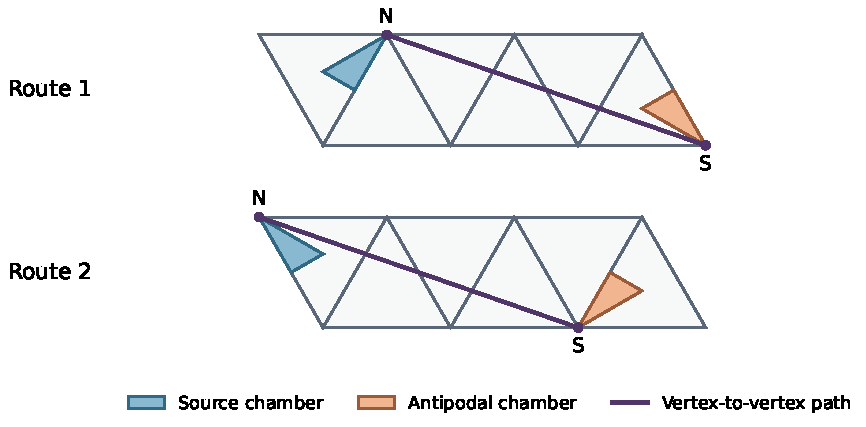
\includegraphics[width=.78\linewidth]{figures/ico_strips.pdf}
\caption{Two developments of the icosahedral surface. Each of the two
shaded triangles is a flag chamber. The displayed segments join
opposite vertices; every choice of a point in each shaded chamber also
gives a valid segment in the corresponding parallelogram.}
\end{figure}
Let $L_1,L_2$ be the two developed segment lengths. The matrix of
$(L_1^2+L_2^2)/2$ on the nine corner pairs, with rows indexed by $C$,
is
\[
 \begin{pmatrix}
 7&13/2&41/6\\ 13/2&25/4&19/3\\ 41/6&19/3&19/3
 \end{pmatrix}.
\]
For barycentric coordinates $\lambda_i$ and $\mu_j$ in the two
chambers, each developed displacement is the weighted sum of the
nine corner displacements with weights $\lambda_i\mu_j$. Convexity
of $Q$ bounds the average by the corresponding weighted sum of the
displayed matrix. The shorter route consequently has squared length at
most $7$. The gap from $7$ in every entry except the upper left is at
least $1/6$, so the same proof gives
\[
 d(x,y)^2\leq 7-\tfrac16(1-\lambda_1\mu_1),
\]
where the subscript $1$ denotes the vertex corner. In particular,
$N,S$ attain the bound. Equality for an arbitrary pair, after folding,
requires both chamber points to be vertices. The chamber isometries
preserve vertex type. Any two distinct nonantipodal vertices can be
joined by at most two unit edges, as the ring labels show, so only
the six unordered antipodal vertex pairs attain diameter. In
particular $S$ is the unique farthest point from $N$.
